%%% Time-stamp: <mainrep.tex 19:57, 17 Jul 2016 by P Sunthar>
%%% $Log:$
% This document describes how to use iitbreport style
%********************************************************************

%\documentclass[11pt,a4paper,openright]{report}
\documentclass[twoside]{iitbreport}

%% Default spacing: 1.5
%% Default font size: 12pt
%% Default font: txfonts (similar to times new roman) 

%% Selectively comment out sections that you want to be left out but
%% maintaining the page numbers and other \ref
\includeonly{%
  intro/introduction,
  assumption/assumption,
  implementation/main,
  lit/literature,
  expt/experimental,
  evaluation/evaluation,
  future_work/future_work,
  rnd/results, 
  dec,abs,pub,ack
}

%%% Some commonly used packages (make sure your LaTeX installation
%%% contains these packages, if not ask your senior to help installing
%%% the packages)

\usepackage{multirow}
\usepackage{booktabs}
\usepackage{listings}
\usepackage{graphicx,array}
\usepackage{epstopdf}
\usepackage{svg}
\usepackage{subcaption}
\usepackage{url}
\captionsetup{subrefformat=parens} % will result in references (typeset with \ref) like  1a  but sub-references (typeset with\subref) like  (a)
\graphicspath{{expt/}}


%%% Macro definitions for Commonly used symbols
\newcommand{\Rey}{\ensuremath{\mathrm{Re}}}
\newcommand{\avg}[1]{\ensuremath{\overline{#1}}}
\newcommand{\tenpow}[1]{\ensuremath{\times 10^{#1}}}
\newcommand{\pder}[2]{\ensuremath{\frac{\partial#1}{\partial#2}}}

% Referencing macros
\newcommand{\Eqref}[1]{Equation~\eqref{#1}}
\newcommand{\Tabref}[1]{Table~\ref{#1}}
\newcommand{\Figref}[1]{Figure~\ref{#1}}
\newcommand{\Appref}[1]{Appendix~\ref{#1}}
%\newcommand{\dime}{{DiME~}}
\newcommand{\dime}{{DiME}}
\newcommand{\isep}{-2 pt}


\newcommand{\subfigANDtitle}[2][.2\linewidth]{%
	\begin{tabular}{@{}>{\centering\arraybackslash}p{#1}@{}} #2 \end{tabular}
}


\begin{document}
	
%%********************************Frontmatter***********************
% In frontmatter everything comes with roman numbering	
\pagenumbering{roman}
\setcounter{page}{1}

%*******************************************************************
%                         Title Page                            
%*******************************************************************
\title{DiME: A Performance Emulator for Disaggregated Memory Architectures}
\author{Abhishek Ghogare}

%% Print the date. Today's date comes by default, change it here to 
%% other date format, if required:

%\date{\today}
\date{October 2017}


%% The type of the report can be set here

\reporttype{Master's Thesis Phase I}
%\reporttype{A Thesis}
%\reporttype{A Dissertation}
%\reporttype{A Project Report}

%% Name of the degree
\degree{Master of Technology}
%\degree{Master of Technology}


%% Department/Centre Name
\dept{Department of Computer Science and Engineering}

%% Supervisor and cosupervisor/excosupervisor are not essential parts
%% of a report title page, as it is your report!

%% But if you **have** to put it uncomment these
%\supervisor{Supervisor name}
%\cosupervisor{Co-super name}
%\excosupervisor{External Supervisor}

%% Roll number
\rollnum{Roll No. 153059006}

\maketitle

%*******************************************************************
%                        Certificate Page                         
%*******************************************************************
%\makecertificate[change title name]{report type} 
%\makecertificate{R\&D report} 
\makecertificate{master's thesis}
%\makecertificate{dissertation}
%\makecertificate{project report}

%\addintoc{Certificate}

%*******************************************************************
%                         Approval Sheet                         
%*******************************************************************
%\makeapproval{thesis}
%\makeapproval{dissertation}

%*******************************************************************
%                          Declaration                           
%*******************************************************************
%==================================dec.tex================================
%
\begin{Declaration}
\noindent
I declare that this written submission represents my ideas in my own words and where others' ideas or words have been included, I have adequately cited and referenced the original sources. I declare that I have properly and accurately acknowledged all sources used in the production of this report. I also declare that I have adhered to all principles of academic honesty and integrity and have not misrepresented or fabricated or falsified any idea/data/fact/source in my submission. I understand that any violation of the above will be a cause for disciplinary action by the Institute and can also evoke penal action from the sources which have thus not been properly cited or from whom proper permission has not been taken when needed.

%
%
%
%
%
%
%

\DecSign[\today]



%
\end{Declaration}
%========================================================================
















 
%\addintoc{Declaration}

%*******************************************************************
%                         List of publications               
%******************************************************************
%%%
\listofpublications


%\noindent Put your publications from the thesis here. The packages \texttt{multibib} or \texttt{bibtopic} or \texttt{biblatex} or enumerate environment or thebibliography environment etc. can be used to handle multiple different bibliographies in the document.

Dhantu Buragohain, Abhishek Ghogare, Trishal Patel, Mythili Vutukuru, Purushottam Kulkarni.2017. DiME: A Performance Emulator for Disaggregated Memory Architectures. In Proceedings of APSys '17, Mumbai, India, September 2, 2017, 8 pages.

\noindent DOI: 10.1145/3124680.3124731

\noindent Git Repository: \href{https://github.com/networkedsystemsIITB/DiME}{https://github.com/networkedsystemsIITB/DiME} \cite{dimerepo}







%%======================================================================
%%% Local Variables: 
%%% mode: latex
%%% TeX-master: "../mainrep"
%%% End: 







        

%******************************************************************
%                          Abstract                             
%******************************************************************  
%============================= abs.tex================================
\begin{Abstract}
Disaggregating various resources is the recent trend in data center architectures, where resources of same type are disaggregated in resource pools, e.g. compute, storage, network and memory. Disaggregation helps in efficient use of power and resources by sharing among servers based on their usage patterns. Since disaggregated resources are shared over external communication link, it can have significant impact on application performance based on the access pattern. Due to unavailability of disaggregated memory hardware, it is difficult for application developers to evaluate the optimizations. We aim to emulate disaggregated memory for a process, so that application developers can use the emulator in development process for testing purpose to make application more efficient in disaggregated environment. We develop a tool, {\dime}, to have more fine-grained control over emulator configurations compared to previously proposed emulators and show its features and usefulness by extensive testing using popular workloads.
%
%
%
%
%
\end{Abstract}
%=======================================================================

                    

%******************************************************************
%                         Contents list                         
%******************************************************************
%\figurespagefalse
%\tablespagefalse
\makecontents % Creats toc, lof, and lot


%%********************************Mainmatter***********************
% In mainmatter everything comes with arabic numbering	
\cleardoublepage
\setcounter{page}{1}
\pagenumbering{arabic}

%******************************************************************
%                         Chapters                           
%****************************************************************** 

\newcommand{\etas}{\ensuremath{\eta_{\mathrm{s}}}}


\chapter{Introduction}

Traditional datacenters are built of collection of servers, and each server has dedicated resources, which are memory, cpu, non-volatile storage (SSD, HDD), network, etc. Per-server memory demands are increasing due to large-memory applications. Leading to more power to operate the memory. A new memory architecture is required to efficiently use the available memory. By disaggregating memory, multiple compute blades can connect to a single memory blade and dynamically share its capacity, resulting in decreased memory requirement and lower power consumption.

We have produced a linux kernel module which tracks the memory accesses by a process and emulates the delay caused by transferring remote memory data to local memory.



%%


%%% Local Variables: 
%%% mode: latex
%%% TeX-master: "../mainrep"
%%% End: 


\chapter{Architecture Assumptions}

We have built the module based on following disaggregation architecture. 
A server has a small amount of local memory. Rest of the memory is located on remote memory "blade". When CPU needs to access an address from an address space which is located on remote memory, it requests it though standard hardware protocol. High speed network interconnection is used to setup communication between devices. A local page is evicted based on the eviction policy. Then the requested remote page is transferred over the network to the local memory. 

\begin{figure}[tbp]
  \centering
    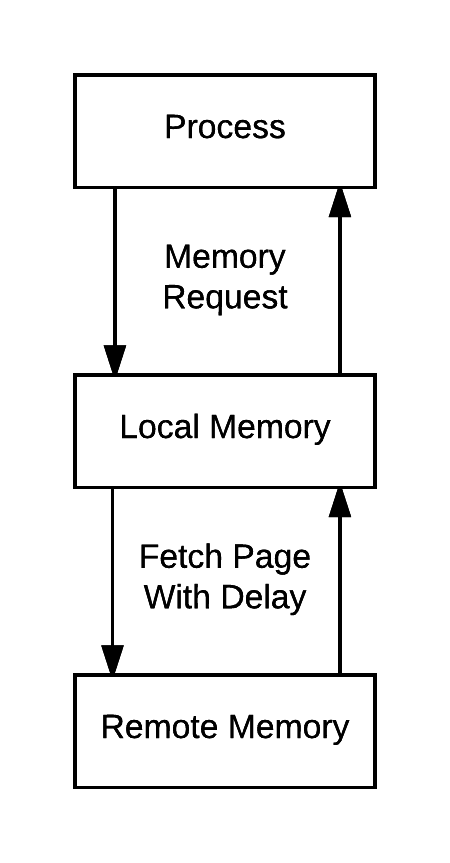
\includegraphics[width=0.25\textwidth]{assumption/architecture_assumption}
    \caption[Disaggregated Memory Flow]{Disaggregated memory flow.}
    \label{fig:arch} 
\end{figure}

%%% Local Variables: 
%%% mode: latex
%%% TeX-master: "../mainrep"
%%% End: 


\chapter{Linux Kernel Background}

\section{Memory Management in Linux}
Linux adopts a paging model to manage memory. Physical memory is divided into pages for more efficiency. A separate page table is maintained for each process which contains page table entries (PTE). PTE stores the actual physical address of the page along with various flags (Table \ref{tab:pte_flags}). PTE of a linear address is extracted from page table by doing a page table walk. Since these translations of linear address to physical address are very time expensive tasks, they are kept in translation lookaside buffer (TLB). In x86 architecture, the page table walk is done by special hardware, memory management unit (MMU). When a TLB miss occurs, the MMU has to populate the TLB entry by doing page table walk. In some architectures where MMU is not present, a page fault is generated in case of TLB miss and kernel page fault handler has to do the translation and update TLB entries. Figure \ref{fig:mmu} shows the memory access flow. A page fault is raised in case of various scenarios where it needs special handling, e.g. PTE not present, invalid page access, invalid PTE, etc.

Since module has to inject the delay at a memory access, page fault handler is the place where we can put the delay logic. When MMU cannot serve the address translation request, a page fault is raised. CPU breaks the normal program execution flow and handles the raised fault. In x86 architecture, function named "\verb|do_page_fault|" in file "arch/x86/mm/fault.c" in kernel source code handles the page fault.

There are various reasons for triggering a page fault. We are going to focus on following reasons:
\begin{enumerate}
	\item Page does not exists, i.e. first reference to the address within the page: demand paging
	\item Page is present in memory and protection bit is set in PTE
	\item Page was swapped-out from memory
\end{enumerate}

If MMU is able to translate the virtual address successfully, no fault is raised and program flow is not interrupted.

\begin{figure}[tbp]
	\centering
	%    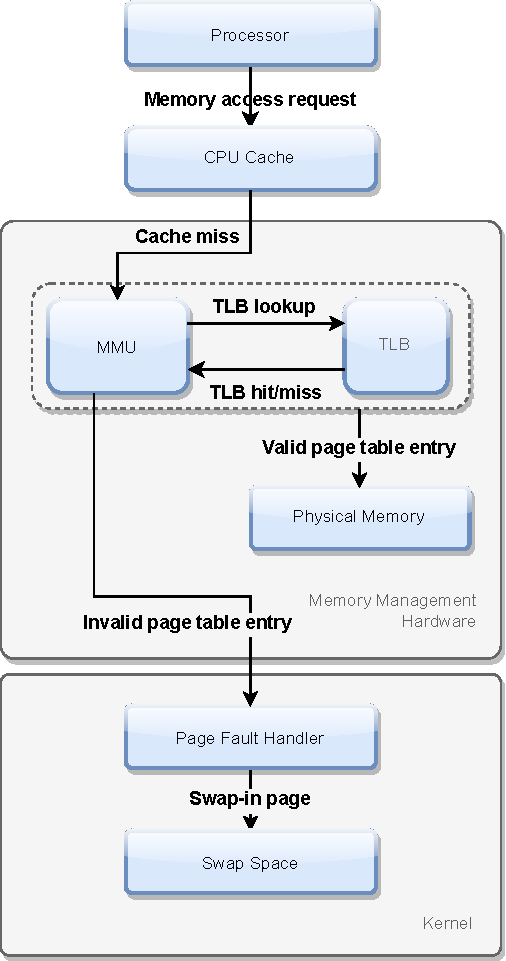
\includegraphics[width=0.5\textwidth]{implementation/mmu.pdf}
	%    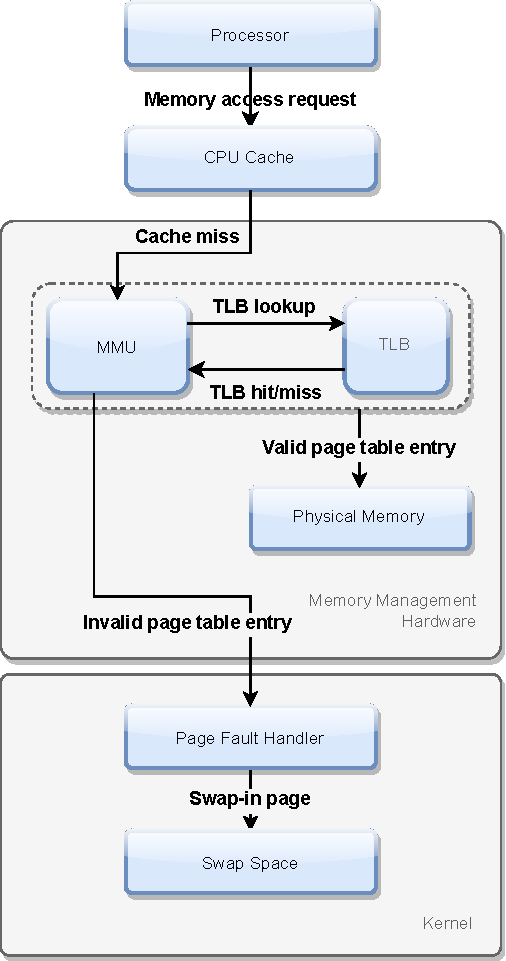
\includegraphics[height=\textheight]{implementation/mmu.pdf}
	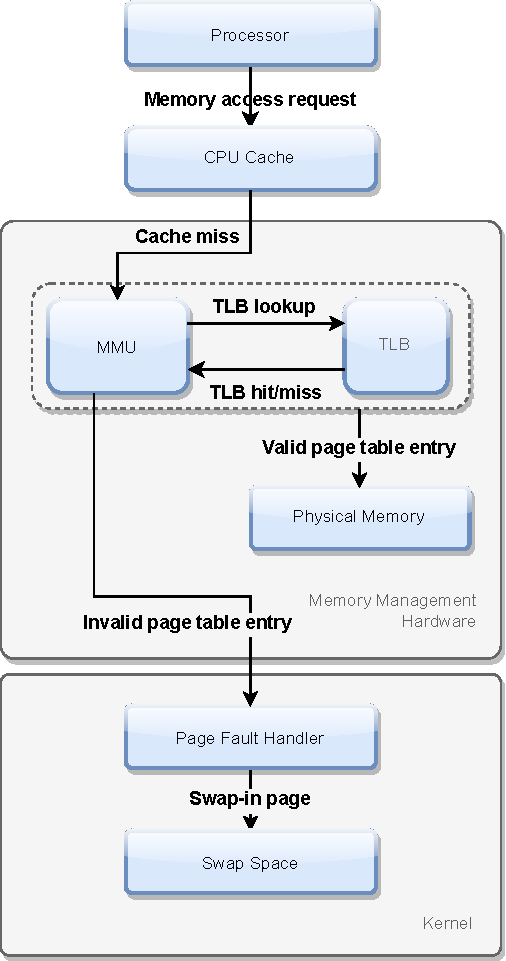
\includegraphics[]{implementation/mmu.pdf}
	\caption[MMU hardware]{MMU and page fault handler interaction.}
	\label{fig:mmu} 
\end{figure}


\begin{table}[tbp]
	\centering
	\caption{PTE flags.}
	\label{tab:pte_flags}
	\begin{tabular}{ll}
		\toprule 
		Bit & Function \\
		\midrule
		\verb|_PAGE_PRESENT| & Page is resident in memory and not swapped out \\
		\verb|_PAGE_PROTNONE| & Page is resident but not accessible \\
		\verb|_PAGE_RW| & Set if the page may be written to \\
		\verb|_PAGE_USER| & Set if the page is accessible from user space \\
		\verb|_PAGE_DIRTY| & Set if the page is written to \\
		\verb|_PAGE_ACCESSED| & Set if the page is accessed \\
		\bottomrule
	\end{tabular}  
\end{table}


\section{Types of Page Faults}

\subsection{Minor Page Faults}
A minor page fault occurs only when a page table is updated (and the MMU configured) without actually needing to access the disk. This happens when a page is shared across processes but current process does not have access for it, e.g. when two or more users use a program at the same time, the text section pages are shared to increase efficiency.

Another example is copy on write. When a new process is forked, the child process shares the address space of parent process. A separate copy of the page is created only when a write operation happens on the shared page.
Both of these page faults has less work to do and page fault occurs only once for that page.

\subsection{Demand paging}
In this case, the page is not present in physical memory and kernel should allocate the page or load the page from disk.
The \verb|_PAGE_PRESENT| flag is not set in PTE. So we can simply add these pages to local page list and execute delay. Two page faults are triggered for this case. First page fault starts loading and allocating the page and second page fault initializes PTE. The \verb|_PAGE_PRESENT| bit is not set in first page fault, but it is set in second page fault. So by checking \verb|_PAGE_PRESENT| only, we can serve multiple page faults for a page only once.

\subsection{Swap-in Pages}
When a page is swapped-in into the memory, its \verb|_PAGE_PROT_NONE| and \verb|_PAGE_PRESENT| flags are reset. So the module has no idea about whether the page was in local page list or not. The only way to find out that is to traverse the list. The size of the list could be very large depending on max number of allowed local pages. Same as demand paging, this type of page fault also triggers two page faults.

There are extra unused bits (\verb|_PAGE_BIT_SOFTW{1,2,3,4}|) of PTE in x86 architecture. We tried setting these bits to represent if page is in local memory or remote memory, but same as \verb|_PAGE_PROT_NONE| bit, they also gets cleared when page gets swapped-in.

Currently we are assuming the physical memory is large enough to accommodate the process and swap space is not used. Current module treats all pages as remote memory for which \verb|_PAGE_PRESENT| is not set and injects the delay.


\begin{table}[tbp]
	\centering
	\caption{PTE flags and corresponding type of page fault.}
	\label{tab:pte_flags_vs_type} 
	\begin{tabular}{cc|p{.2\textwidth}|p{.3\textwidth}}
		\toprule 
		\multicolumn{2}{c|}{Bits} &  
		\multirow{2}{*}{Type} & \multirow{2}{*}{Action} \\
		%	\cline{1-2}
		\_PAGE\_PRESENT& \_PAGE\_PROT\_NONE & &     \\
		\midrule	
		0 & 0 &  Page not present in physical memory & 
		Check page in local page list, add if not present and emulate delay		
		\\ \hline		
		0 & 1 &  
		Page is present but protected 		&  
		Add to local page list and emulate delay \\ 
		\hline	
		1   & 0     & Page is loaded in physical memory, but not initialized & Ignore page fault, since page is already in local page list
	\end{tabular}
\end{table}


\chapter{Design and Implementation}

\section{Overall Design}
{\dime} is built of two primary parts, a single core module and multiple page replacement policy modules. When a page fault gets triggered, the core module checks if the concerned process is running inside the emulator. The page fault information is then forwarded to the page replacement policy module which does the necessary bookkeeping and evicts a local page to make a spare slot available for the remote page. At the end, core module receives a signal whether to inject delay or not.

{\dime} takes a list of PIDs for which remote memory is to be emulated along with other configuration parameters, i.e. number of local pages, one-way latency, network bandwidth (Table \ref{tab:kmodule_param}). {\dime} logically divides the process memory into two parts: local and remote. {\dime} injects delay whenever a remote memory page is accessed. Delay is propagation and transmission delays to fetch the remote page. We will refer both combined as "delay" in rest of the report. Transmission delay is calculated based on network bandwidth and the size of the page that is being fetched.


\section{Emulator Work-flow}
To emulate remote memory, {\dime} protects a portion of virtual address space of processes under emulation which corresponds to remote memory so that when a protected page is accessed, it will trap to the page fault handler and delay will be injected. {\dime} supports multiple emulator instance feature, which enables different process groups to be emulated on separate remote memory, network architecture and page replacement policy simultaneously.

To inject the delay to each page fault, {\dime} follows the steps :
\begin{enumerate}
	\item Intercept "\verb|wake_up_new_task|" function calls to check if new process was forked by any of the tracking processes
    \item Intercepts each page fault
    \item Determine if the page fault is raised for a process for which the emulation is running
    \item Determine if the faulted address is in the local memory or the remote memory
    \item No delay injection if address belongs to local memory
    \item If address is in remote memory, forward page fault information to page replacement policy module
    \begin{enumerate}
        \item If local memory pool is free, virtually allocate the new local page to the faulted page
        \item Else virtually evict and protect a page from local memory pool and allocate the new freed slot to the faulted page
        \item Instruct core module whether to inject delay or not
    \end{enumerate}
    \item Inject the delay for emulating the transmission and propagation delays
\end{enumerate}



\section{Intercept Page Fault Handler}
Module needs to intercept each page fault so that it can emulate the delay. There are two ways to intercept a kernel function:
\begin{enumerate}
	\item KProbe
	\item Kernel hooks
\end{enumerate}

\subsection{KProbe}

KProbe \cite{kprobe} is a debugging mechanism provided by the kernel to track activities inside kernel. A kprobe can be registered to any function whose address is known at the time of kprobe insertion. Major benefit of using kprobes is that kernel recompilation is not needed and can be registered on live kernel through kernel module.

In Linux kernel, \verb|do_page_fault| function has to read CR2 register which contains page fault linear address before any other tracing mechanism get called to properly handle the page fault. Therefore, \verb|do_page_fault| is blacklisted from kprobe and tagged as notrace. Hence we are left with kernel hooks option to intercept page fault handler.

\subsection{Kernel hooks}
Adding a hook to the kernel function is another way of intercepting a function call, but with added overhead of kernel recompilation. We have added a hook function pointer in \verb|fault.c| file initialized to null value. We are calling the hook function before \verb|__do_page_fault| function in \verb|do_page_fault| function. The hook function is called only if the function pointer is not null. The hook function pointer is exported so that the kernel module can set its value to pointer to custom function defined inside the module. Module sets the hook function pointer back to null at the time of module removal, to prevent invalid memory access.

Listing \ref{list:hooks} shows how hook function pointers are declared, exported and called from page fault handler.

\begin{lstlisting}[
language=C,
backgroundcolor=\color{lightgray},
caption={Hook functions in fault.c},
label=list:hooks,
basicstyle=\footnotesize]
int (*do_page_fault_hook_start)(struct pt_regs *regs,
                                unsigned long error_code,
                                unsigned long address) = NULL;
EXPORT_SYMBOL(do_page_fault_hook_start);

int (*do_page_fault_hook_end)(struct pt_regs *regs,
                              unsigned long error_code,
                              unsigned long address) = NULL;
EXPORT_SYMBOL(do_page_fault_hook_end);

dotraplinkage void notrace
do_page_fault(struct pt_regs *regs, unsigned long error_code) {
    unsigned long address = read_cr2(); /* Get the faulting address */
    enum ctx_state prev_state;
    
    // Calling do_page_fault_hook_start hook function
    if(do_page_fault_hook_start != NULL) {
        do_page_fault_hook_start(regs, error_code, address);
    }

    prev_state = exception_enter();
    __do_page_fault(regs, error_code, address);
    exception_exit(prev_state);

    // Calling do_page_fault_hook_end hook function
    if(do_page_fault_hook_end != NULL) {
        do_page_fault_hook_end(regs, error_code, address);
    }
}
\end{lstlisting}


\section{Induce Page Faults}

In Linux, a page fault can be induced for any future access to the page by setting the \verb|_PAGE_PROT_NONE| bit and resetting \verb|_PAGE_PRESENT| bit of PTE of the required page. This combination of bits prevents page fault handler from behaving unexpectedly and still make MMU to raise a page fault. It suggests that the page is present in memory but access to it is protected. Setting the above combination of flags is referred as protecting the page and setting opposite combination of flags (i.e. \verb|_PAGE_PROT_NONE|=0 \& \verb|_PAGE_PRESEN|=1) is referred as releasing the page in rest of the report for simplicity.
{\dime} protects all pages of the emulating processes at initialization. This way every memory access by the given processes will trigger the page fault.


\subsection{TLB \& Cache Flush} \label{ssec:tlb_flush}
In x86 architecture, it is specified that TLB cache are not coherent with page table (cache and TLB flush \citep{cachetlb}). It is possible to exists stale translation entries in TLB after page table is altered. Therefore it is necessary to flush relevant TLB entries when page table entry is updated. 

In general, when virtual to physical address mapping is changed or a page table entry is updated following actions are required to take:
\begin{enumerate}
	\item Flush CPU cache
	\item Update page table entry
	\item Flush TLB
\end{enumerate}

CPU cache flush is required to be first, because it helps to properly handle architectures which strictly requires valid address translation to exist for a virtual address before that address is flushed.

In {\dime}, it is required to flush TLB after a page is protected, because even if we protect a page in page table, it is possible to exist stale entry in TLB which would serve the address translation and page fault would not raise. We explain the test case where TLB flush is essential in section \ref{ssec:cache_flush_eval}.

{\dime} first initializes the required data structures and sets up the hooks before protecting the pages so that it will not miss any page fault.

\begin{figure}[tbp]
  \centering
    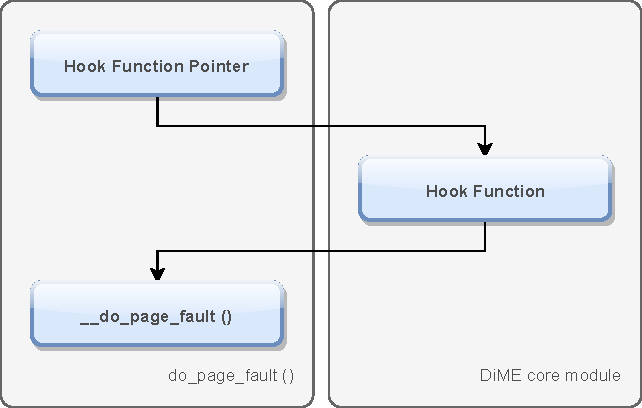
\includegraphics[width=0.7\textwidth]{implementation/hook.pdf}
    \caption[Hook Function]{Hooking a page fault handler function.}
    \label{fig:hook_1} 
\end{figure}


\section{Delay Injection} \label{sec:delay_injection}
Now we have setup the page fault interception and induced the page fault for every memory access from the insertion of our module, which is our first step. The delay injection logic is implemented in the hook function defined in the module.

Linux kernel provides different ways to introduce a delay in an execution flow, viz. \verb|delay| and \verb|sleep| function families~\cite{timers}. The sleep function family is backed by high-resolution kernel timers subsystem. The \verb|usleep_range| function takes a time range and schedules a wakeup event anywhere in the range before sleeping. As an optimization, it coalesce wakeup with any other wakeup that may have happened for other reasons. At the worst case, a new wakeup event is scheduled at the upper bound of the time range. Due to this involvement of the wakeup scheduling and interrupt mechanism, it cannot be used for injecting small delays (e.g., a few hundred nanoseconds) precisely. The delay function family is backed by a busy-wait loop which executes the desired delay by iterating a single instruction which approximately takes 1$\mu$s. Since the execution time of this instruction is not exactly 1$\mu$s, but has some positive error, the error gets accumulated for a large number of iterations. Therefore, the delay injection error is less for delays close to 1$\mu$s, but increases linearly for higher delays. Because of the limitations of the above two techniques, {\dime} uses a custom busy-wait implementation backed by \verb|sched_clock| function to enforce delays. The \verb|sched_clock| function uses the system jiffies counter internally. The module checks the timestamp using \verb|sched_clock| function and iterates in a loop until the elapsed time is less than the delay to be executed. We used a custom busy-wait loop as our delay injection method since it provides the highest accuracy with a constant small error for a broad range of delays. Comparison of delay accuracy is discussed in Section \ref{ssec:delay_eval}.

\begin{table}[]
	\centering
	\caption{Delay function families}
	\label{delay_functions}
	\begin{tabular}{lll}
		\hline
		\textbf{Function}     & \textbf{Idle for interval} & \textbf{Backed by}       \\ \hline
		ndelay                & \textless$\sim$1000$ns$     & busy-wait loop on jiffie \\
		udelay                & \textless $\sim$10${\mu}s$ & busy-wait loop on jiffie \\
		mdelay                & -                          & udelay                   \\
		usleep\_range         & 10${\mu}s$ - 20$ms$                & hrtimers                 \\
		msleep                & 10$ms$+                      & jiffies / legacy\_timers \\
		msleep\_interruptible & 10$ms$+                      & jiffies / legacy\_timers \\ \hline
	\end{tabular}
\end{table}


\section{Page Replacement Policy}
A local page is evicted from local memory to accommodate the remote page for which page fault is raised. A page replacement policy decides which local page to evict next. {\dime} provides an API to register/deregister a separate page replacement policy module, so that users can write their own local page list management mechanism and have control over which page to evict based on their own algorithm. This way user do not need to rely on default algorithm provided by operating system and can experiment with custom algorithms. We have implemented a simple FIFO policy for testing and illustrative purpose, which is used for all evaluations described in this document.

\subsection{Policy structure hierarchy design}
To implement custom policy module, user needs to implement functions described in \verb|struct page_replacement_policy_struct| and pass this \verb|struct| to core module while registering the policy. To avoid casting a void pointer with different policy structure types, user can use \verb|container_of| macro to extract the pointer to parent policy \verb|struct| from pointer to \verb|struct page_replacement_policy_struct|. E.g., as shown in figure \ref{fig:class_diagram}, pointer to object of type \verb|struct prp_fifo_policy| can be derived from pointer to member object \verb|prp| as follows:

\begin{center}
	\verb|container_of(prp, struct prp_fifo_struct, prp);|
\end{center}

Since the policy functions have information about the type of policy structure, we neither need to maintain a void pointer to policy struct nor unsafe casting it to the actual type.

\begin{figure}[tbp]
	\centering
	%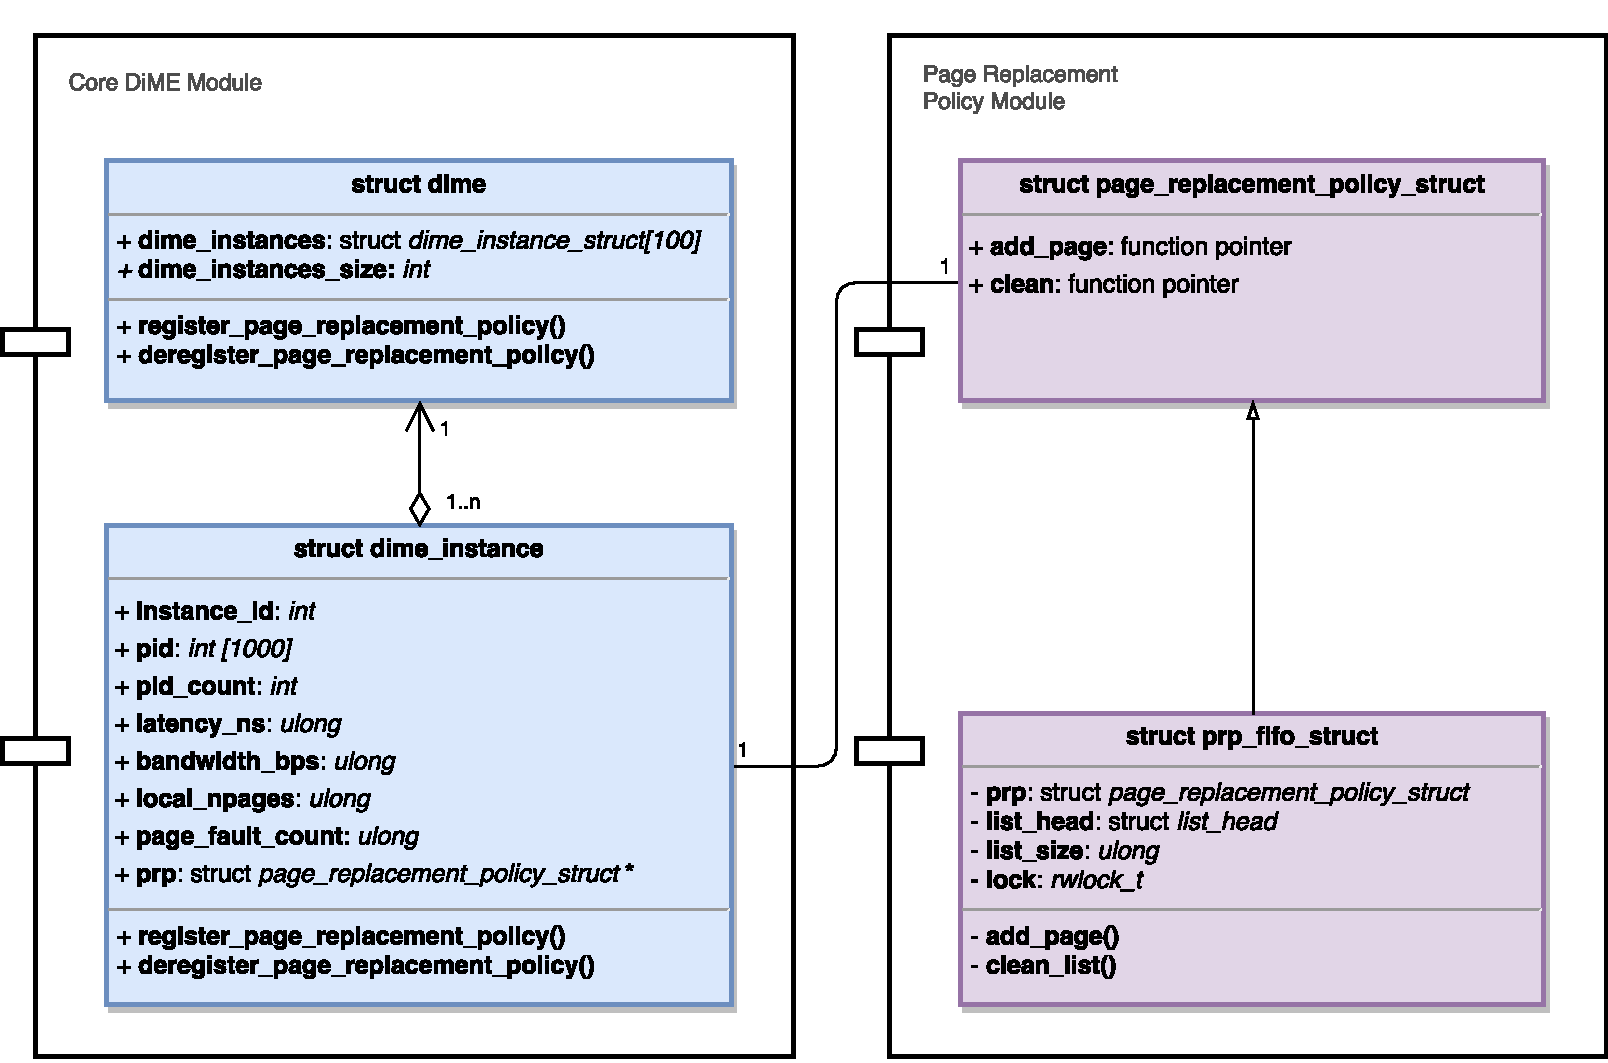
\includegraphics[width=0.5\textwidth]{implementation/class_diagram.pdf}
	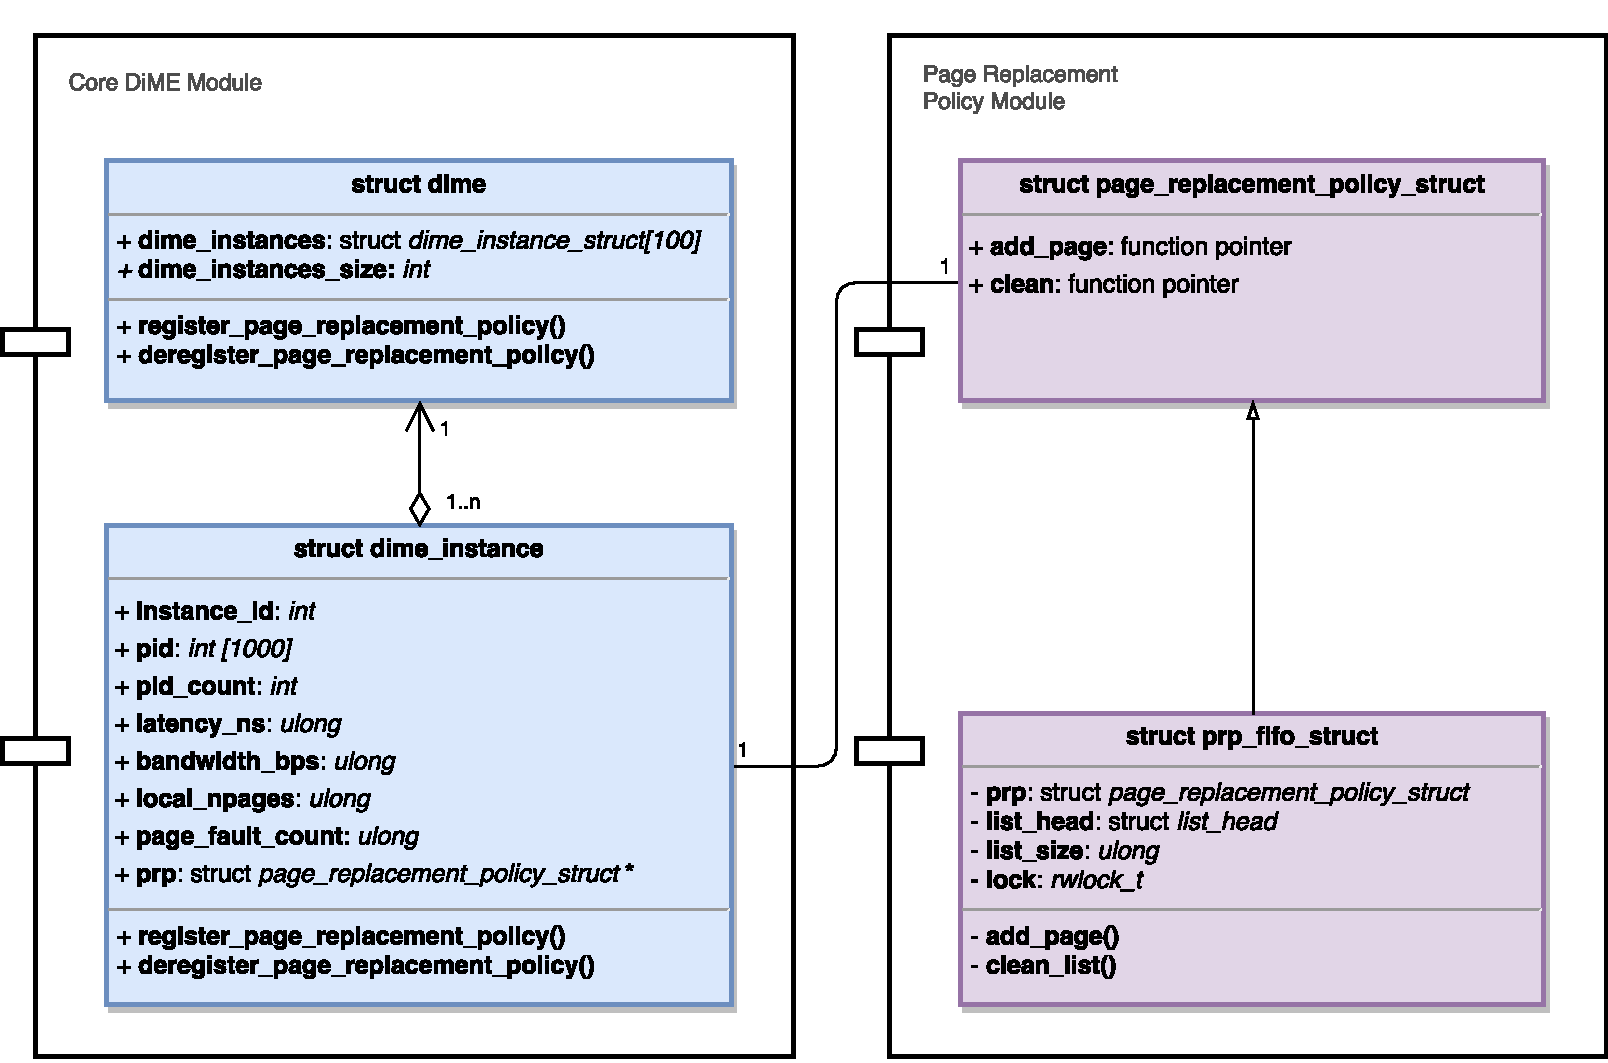
\includegraphics[width=\textwidth]{implementation/class_diagram.pdf}
	\caption[Class Diagram]{Page replacement policy class diagram}
	\label{fig:class_diagram} 
\end{figure}


\subsection{Virtual memory location}
It is responsibility of policy to maintain a list of local pages, handle a remote page fetch request and signal whether to inject delay to this page fault based on location of the requested page.
Local pages are virtually at the local memory for which page fault will not raise. Local page list helps to select a local page for eviction. To make a spare slot for remote page, a local page is protected and removed from the local page list, so that any future reference to that page would raise a page fault.

\section{Second Hook}

\subsection{Accurate delay execution}
The hook function can take variable amount of time to reach at the delay execution code based on the various tasks it needs to complete, e.g. local page lookup, update, etc. Also, \verb|__do_page_fault| function can take variable time to return based on the type of page fault. Therefore, there will be variable amount of delay injection for each page fault.

To be able to inject the exact amount of delay based on the configuration parameters, the module must calculate the time spent on these extra tasks and inject delay worth of the difference of desired delay and time spent.
To achieve the accurate delay execution, we need another hook function which will be called at the end of \verb|do_page_fault| function. Now the first hook function will take the timestamp as a start of the handler and the second hook function will execute the difference worth of delay at the end.

The timestamp variable must be accessible from both hook functions, but it should not be taken as a global variable, since there might be multiple page faults being handled at the same time. So, we declare a timestamp variable in \verb|do_page_fault| function, whose single instance will be common for both hook functions but different for each page fault.

\subsection{Delay execution decision}
The page replacement policy can take decision whether the faulted page is in local or remote memory based on the policy rules that are configured by the user, e.g. pin a portion of memory to local, mark data section of a process as always remote, etc. The delay injection depends upon this decision.

Now again since both hooks are different functions, we cannot have a global flag variable for the decision communication. So, same as timestamp, we declare a flag variable in \verb|do_page_fault| and its pointer is sent to both hooks as an argument.

\begin{figure}[tbp]
  \centering
    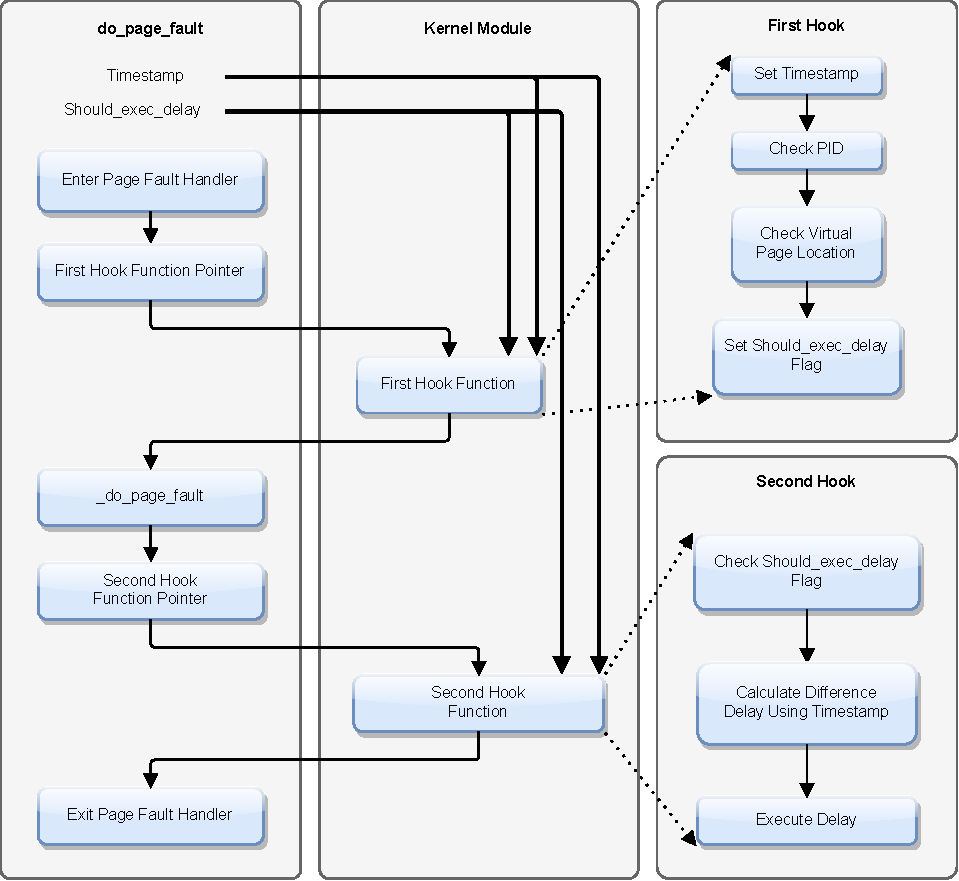
\includegraphics[width=1.0\textwidth]{implementation/second_hook.pdf}
%    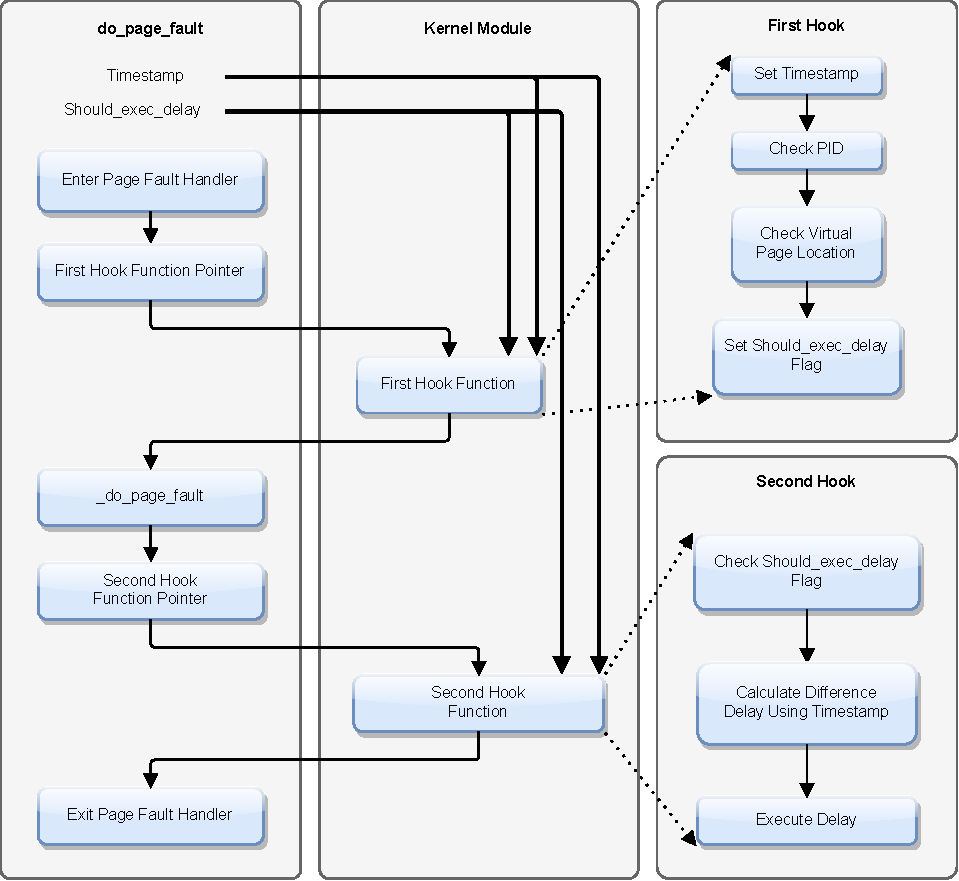
\includegraphics[]{implementation/second_hook.pdf}
    \caption[Second Hook Function]{Emulator with second hook.}
    \label{fig:hook_2} 
\end{figure}

\section{Multiple Emulator Instances Design}
{\dime} allows users to run multiple emulator instances simultaneously. The instances has separate local memory and can be configured with different configuration parameter set. This feature is helpful to emulate different processes with different relative location of remote memory, e.g. rack scale or across data center.

\section{Track Processes Under Emulator}
\subsection{TGID}
{\dime} instance maintains a list of PIDs of processes which are running under that emulator instance. For each page fault, {\dime} checks the faulting PID in all running {\dime} instances to determine to which instance this PID belongs. In Linux kernel, the PIDs of threads that belong to same process are different, but \verb|tgid| (thread group ID) is same as the parent thread. Therefore, we use \verb|tgid| of "\verb|current|" \verb|task_struct| rather than \verb|pid| to track the process.

\subsection{Process forks}
It is possible that a process running under emulator might fork a new thread or process. The expected behavior is that the new process should also run under the same {\dime} instance which contains the process which forked it. Since we are tracking based on thread group ID, forking a new thread satisfies the expectation. In case of a process, we need to add its PID to that {\dime} instance.

Linux kernel function \verb|wake_up_new_task| wakes up a newly forked process after all the process initialization is done. To track process forks, {\dime} registers a KProbe~\cite{kprobe} to \verb|wake_up_new_task| and every time a new process is forked it check if the parent of new process belongs to any of the running {\dime} instances. If found, the new PID is appended to the PID list and all its pages are protected.


\section{Dynamic Configuration}
{\dime} supports dynamic modification of configuration parameters (Table \ref{tab:kmodule_param}) and add new emulator instances. A proc file, "\verb|\proc\dime_config|", is implemented to handle the dynamic configuration change requests. 

\scriptsize
\begin{lstlisting}[
%language=bash,
backgroundcolor=\color{lightgray},
caption={Procfs based {\dime} configuration example},
label=list:dime_config,
basicstyle=\ttfamily,breakatwhitespace=true,breaklines=true,framextopmargin=50pt,frame=bottomline
]
$ echo "instance_id=1 latency_ns=500 bandwidth_bps=1000000000 local_npages=5000 pid=8765,4321" > /proc/dime_config
$ cat /proc/dime_config
instance_id latency_ns bandwidth_bps local_npages page_fault_count pid
          0       1000    1000000000         2000                0 1234,5678,
          1        500    1000000000         5000                0 8765,4321,
\end{lstlisting}
\normalsize

\begin{table}[]
	\centering
	\caption{{\dime} config parameters in /proc/dime\_config }
	\label{tab:kmodule_param}
	\begin{tabular}{ll}
		\hline
		\textbf{Parameter name} & \textbf{Use} \\ \hline
		\verb|instance_id| & Instance ID of the target {\dime} instance \\
		\verb|latency_ns| & One-way propagation delay in nano-seconds \\
		\verb|bandwidth_bps| & Network bandwidth in bits per seconds \\
		\verb|local_npages| & Available local memory in number of pages \\
		\verb|page_fault_count| & Number of page faults raised till now \\
		\verb|pid| & A comma separated list of PIDs to add under emulator \\ \hline
	\end{tabular}
\end{table}

%%% Local Variables: 
%%% mode: latex
%%% TeX-master: "../mainrep"
%%% End: 

\chapter{Evaluation}
This section describes {\dime} accuracy and comparison with other emulator.
All experiments were performed on an Intel Xeon CPU E5-2650 server with 16 hyper-threaded and CPUs operating at 2.60 GHz. Each application was executed from within a Linux/KVM virtual machine with 3 vCPUs and 6 GB RAM running Linux kernel 4.4.70 with huge page disabled.

\section{Verification of Correctness}
We evaluated {\dime} for correctness based on different scenarios and test cases.

\subsection{Page faults}
We have written a test program in C language, which takes number of pages as an argument and "malloc"ates the memory. Since we have disabled huge pages, default page size is 4kB. The program first accesses all the allocated pages in sequence and then access last 'x' pages. At the end of execution, test script extracts total number of page faults occurred from {\dime} procfs config file, \verb|/proc/dime_config|.

We setup {\dime} with following configurations: \verb|local_npages|=1000; \verb|latency_ns|=10000; \verb|bandwidth_bps|=10000000000000000 (infinite). We allocate 2000 pages in test program that runs under emulator. Table \ref{tab:last_page_access_test} shows test results where we vary number of last pages accessed ('x') and calculate the page faults. As expected, the number of page faults are constant till x=900, i.e. ~2000 for first iteration of page access, and starts increasing after x=1100 by ~100. It shows that 900 last pages were already in local memory and no page fault raised for those. Since FIFO page replacement policy is used, the page fault count jumps by ~1000 at x=1100, because all local pages are evicted from list once again. The extra ~100 page faults that we see in all test cases are of test program text section which are always required in local memory for program execution.

\begin{table}[]
	\centering
	\caption{Last 'x' pages access test results}
	\label{tab:last_page_access_test}
	\begin{tabular}{cccc}
		\hline
		\textbf{\begin{tabular}[c]{@{}c@{}}Number of last\\ pages accessed\end{tabular}} & \textbf{\begin{tabular}[c]{@{}c@{}}Total execution\\ time (us)\end{tabular}} & \textbf{\begin{tabular}[c]{@{}c@{}}Number of\\ page faults\end{tabular}} & \textbf{\begin{tabular}[c]{@{}c@{}}Average time taken\\ per page fault (us)\end{tabular}} \\ \hline
		0 & 50,989.50 & 2,099.00 & 24.29 \\
		100 & 51,113.50 & 2,102.50 & 24.31 \\
		200 & 51,145.00 & 2,100.50 & 24.35 \\
		300 & 50,733.50 & 2,099.50 & 24.16 \\
		400 & 50,289.00 & 2,100.50 & 23.94 \\
		500 & 49,209.50 & 2,099.50 & 23.44 \\
		600 & 47,617.50 & 2,100.50 & 22.67 \\
		700 & 48,605.00 & 2,102.00 & 23.12 \\
		800 & 49,755.50 & 2,102.00 & 23.67 \\
		900 & 46,625.00 & 2,101.00 & 22.19 \\
		1000 & 53,386.00 & 2,339.50 & 22.82 \\
		1100 & 72,608.00 & 3,182.00 & 22.82 \\
		1200 & 73,316.50 & 3,269.00 & 22.43 \\
		1300 & 77,493.50 & 3,388.00 & 22.87 \\
		1400 & 79,642.50 & 3,491.50 & 22.81 \\
		1500 & 77,371.50 & 3,595.50 & 21.52 \\
		1600 & 82,422.00 & 3,695.50 & 22.30 \\
		1700 & 81,398.50 & 3,801.50 & 21.41 \\
		1800 & 86,171.50 & 3,910.00 & 22.04 \\
		1900 & 84,671.50 & 3,999.50 & 21.17 \\
		2000 & 90,360.50 & 4,107.00 & 22.00 \\ \hline
	\end{tabular}
\end{table}

\subsection{Cache flush requirement} \label{ssec:cache_flush_eval}
As explained in Section \ref{ssec:tlb_flush}, it is mandatory to flush TLB after every page table update. To verify this, we built a C program which allocates 1000 pages, i.e. 1000x4KB memory, and accesses only two bytes from two different pages alternatively 1000 times per byte. We modified {\dime} to protect only the allocated 1000 pages, i.e. only data section of the process and not the text section. We set \verb|local_npages|=1 so that last page always get protected for each page fault. It was found that if we do not flush TLB after protecting previously accessed page, the page fault count was around $\sim$200, which is much less than expected count of 2000. After we patched the module with TLB flush, the page fault count was exactly 2000 as expected.


\subsection{Delay injection accuracy} \label{ssec:delay_eval}
As described in section \ref{sec:delay_injection}, there are multiple ways to inject a delay \cite{timers}. We evaluate each method by injecting delays from 0 to 10000 nanoseconds. In Linux kernel, different clock sources \cite{clock_sources} can be used to measure time \cite{measure_timelapse}. We use Time-stamp counter (TSC~\cite{tsc}) source available in x86 architecture (TSC library \cite{tsclibrary}) to measure actual injection time in each case. We sampled the measurement over 100 times and calculated the average for each method. Figure \ref{fig:lat_accuracy} show the plot between delay injected (x-axis) and actual measured delay (y-axis). The \verb|usleep_range| function deviates most from idle delay injection since it involves interrupts and is nondeterministic delay between the given range. \verb|usleep_range| is not useful for small amount of delays, since the error is higher for delays less than 2000ns. The \verb|ndelay| function injects delay with much higher accuracy for lower values of delay, but the error increases linearly for higher values of delay. Our custom busy loop method of delay injection works most accurately with almost constant error of 70ns for any value of delay.

\begin{figure}[t]
	\centering
	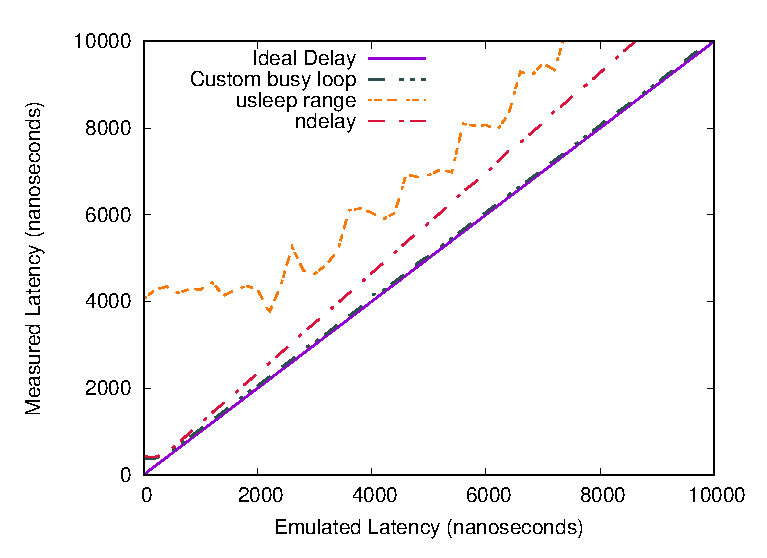
\includegraphics{evaluation/lat_accuracy.eps}
	\caption{Accuracy of delay injection methods.}
	\label{fig:lat_accuracy}
\end{figure}

\subsection{Average time per page fault}
From Table \ref{tab:last_page_access_test}, average time taken per page fault is 22.87${\mu}s$. The expected time was 20${\mu}s$ (two times one-way latency, 2x1000 ns), the error is of 2.87${\mu}s$. Since the time is measured from user space, the error contains context switching and interrupt handling time.


\section{Application Throughput Test}
The application performance degrades which are running under emulator. To verify if performance degradation is valid based on emulator configuration, we vary each parameter by keeping other constant. We ran Redis~\citep{redis} server under emulator with 3 server threads. We used YCSB\cite{ycsb} benchmarking to generate the load. Redis client with 10 client threads, running on another VM, generates 1Gb of workload with equal amount of read and write operations. In Figure \ref{fig:vary_config_localmem}, we vary amount of local memory available for Redis server in percent of workload by keeping network bandwidth and latency constant. Results show that server throughput increases as available local memory increases.

Figure \ref{fig:vary_config_latency} shows the test results where bandwidth and local memory is constant while latency is changed. As we can see, the server throughput increases as latency decreases.

Similar results were observed when Memcached~\cite{memcached} was used in place of Redis.

\begin{figure}[t]
	\centering
	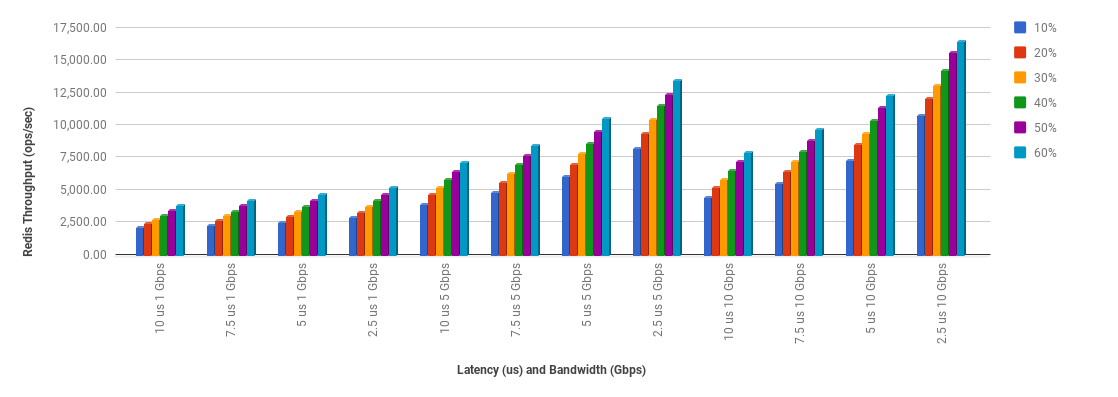
\includegraphics[width=\linewidth]{evaluation/vary_config_throughput_local_mem.png}
	\caption{Redis throughput with constant latency and bandwidth, varying local memory}
	\label{fig:vary_config_localmem}
\end{figure}

\begin{figure}[t]
	\centering
	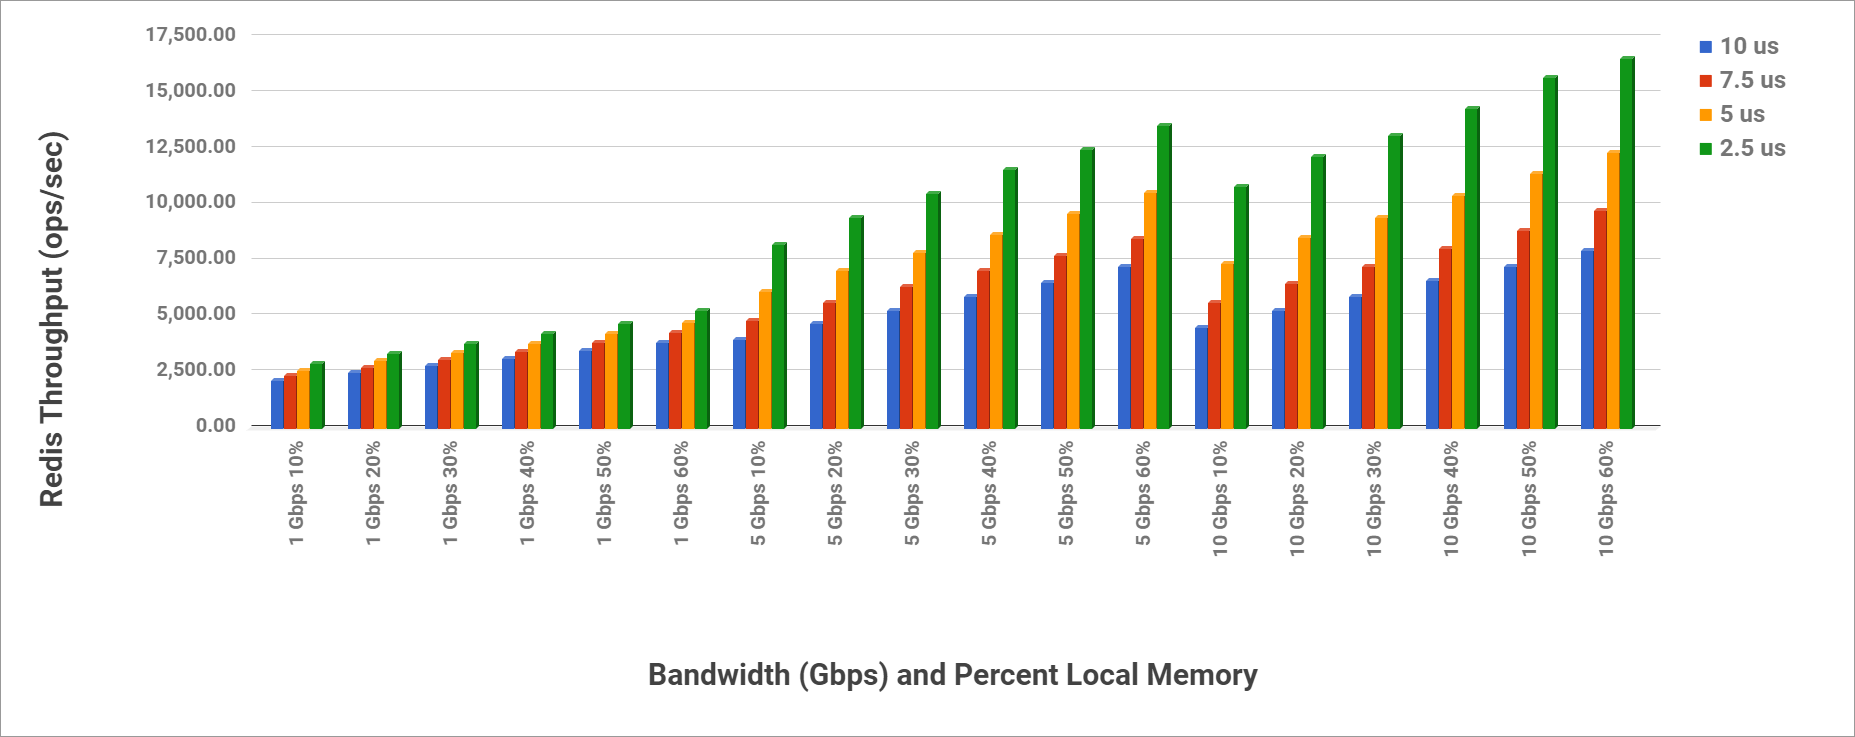
\includegraphics[width=\linewidth]{evaluation/vary_config_throughput_latency.png}
	\caption{Redis throughput with constant bandwidth and percent local memory, varying latency}
	\label{fig:vary_config_latency}
\end{figure}

\section{Comparison with System-wide Emulator}
The existing emulators (e.g. the one developed in \cite{Gao}) emulates memory at system granularity. The entire system memory is partitioned into remote and local memory and user has no control over which portion of memory should reside on remote or local. In contrast, {\dime} emulates remote memory at the granularity of a process. {\dime} also has page level control over amount of local/remote memory and can specify custom page replacement policy. The allocated local memory is fixed and other applications running on the system outside the emulator has no effect on emulation. On the other hand, system-wide emulator cannot eliminate the effect of other applications running simultaneously outside the emulator. There are also other factors which affects the emulation accuracy in case of system-wide emulator, e.g. page cache usage, local memory consumed by other processes running in background, swap-out threshold, etc.

We compare the performance degradation of popular real world applications (Redis~\cite{redis} and Memcached~\cite{memcached}) in case of {\dime} and system-wide emulator\cite{Gao}. In evaluation setup, we vary local memory while keeping latency and bandwidth constant for both emulators. We run multiple tests based on number of instances of application and how they share the local memory described in Table \ref{tab:graph_legends}. Note that we allocate local memory two times in case of shared memory compared to single instance case. 

Figure \ref{fig:compare_pf_redis} shows how number of page faults decreases as local memory increases while Figure \ref{fig:compare_tp_redis} shows how Redis throughput increases as local memory increases. The number of page faults and application throughput is expected to be same in any test scenario described in Table \ref{tab:graph_legends} for a given emulator and a fixed set of configuration parameters. As we can see, in case of {\dime}, all four graphs almost overlap, while in case of system-wide emulator, there is very significant difference. Similar trends are shown by Memcached except the throughput in case of single instance of Memcached server running under {\dime} has more throughput compared to two instances of Memcached. The reason behind this behavior is that, Memcached is more CPU intensive compared to Redis and has more difference in throughput in both cases without any emulator (Table \ref{tab:deg_without_emulator}). The results prove that {\dime} is capable of eliminating any background noise efficiently for more emulation accuracy compared to other emulators. 

\begin{table}[]
	\centering
	\caption{\% Degradation of throughput without emulator}
	\label{tab:deg_without_emulator}
	\begin{tabular}{l|ll}
		\hline
		& Redis & Memcached \\ \hline
		Two instances of server running simultaneously & 30,557.88 & 17,038.53 \\
		Single instance of server running & 35,863.53 & 23,670.20 \\ \hline
		\% Degradation & 14.79\% & 28.02\% \\ \hline
	\end{tabular}
\end{table}

\subsection{Emulator Overhead}
{\dime} has very low overhead of managing local pages since only operation it needs is to set PTE flags. This enables us to emulate low latencies. In a test setup, we set \verb|latency_ns|=0 and infinite bandwidth for both {\dime} and system-wide emulator. We compared total time taken per page fault to execute a simple test program (described previously). Test result populated in Table \ref{tab:emulator_overhead} shows {\dime} has half overhead compared to system-wide emulator.

\begin{table}[]
	\centering
	\caption{Emulator overhead}
	\label{tab:emulator_overhead}
	\begin{tabular}{cccc}
		\hline
		& \textbf{\begin{tabular}[c]{@{}c@{}}Number of page\\ faults observed\end{tabular}} & \textbf{\begin{tabular}[c]{@{}c@{}}Execution\\ time (us)\end{tabular}} & \textbf{\begin{tabular}[c]{@{}c@{}}Time per \\ page fault (us)\end{tabular}} \\ \hline
		\textbf{\begin{tabular}[c]{@{}c@{}}System-wide\\ emulator\end{tabular}} & 2487746 & 19426305 & 7.808797602 \\ \hline
		\textbf{DiME} & 2497209 & 12101210 & 4.845893956 \\ \hline
	\end{tabular}
\end{table}

\begin{table}[]
	\centering
	\caption{Graph Legends for \ref{fig:compare_redis} and \ref{fig:compare_memcached}}
	\label{tab:graph_legends}
	\begin{tabular}{ll}
		\hline
		\textbf{b\_single} & System-wide emulator \cite{Gao} with single instance of application running \\ \hline
		\textbf{b\_shared} & \begin{tabular}[c]{@{}l@{}}System-wide emulator with two instances of application \\ running with shared local memory\end{tabular} \\ \hline
		\textbf{k\_single} & DiME with only one instance of application running \\ \hline
		\textbf{k\_multisingle} & \begin{tabular}[c]{@{}l@{}}DiME with two instances of application running with one under \\ emulator and other outside emulator\end{tabular} \\ \hline
		\textbf{k\_separate} & \begin{tabular}[c]{@{}l@{}}DiME with two instances of application running in separate \\ instances of DiME\end{tabular} \\ \hline
		\textbf{k\_shared} & \begin{tabular}[c]{@{}l@{}}DiME with two instances of application running with shared \\ local memory in one instance of DiME\end{tabular} \\ \hline
	\end{tabular}
\end{table}

\begin{figure}[t]
	\centering
	
	\begin{subfigure}[t]{\textwidth}
		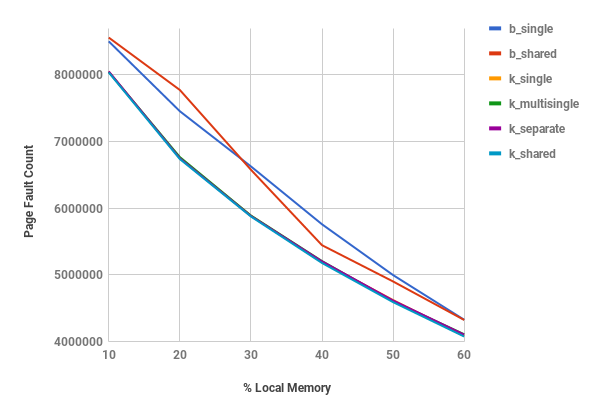
\includegraphics[width=\textwidth]{evaluation/compare_pf_redis.png}
		\caption{}
		\label{fig:compare_pf_redis}
	\end{subfigure}
	\begin{subfigure}[t]{\textwidth}
		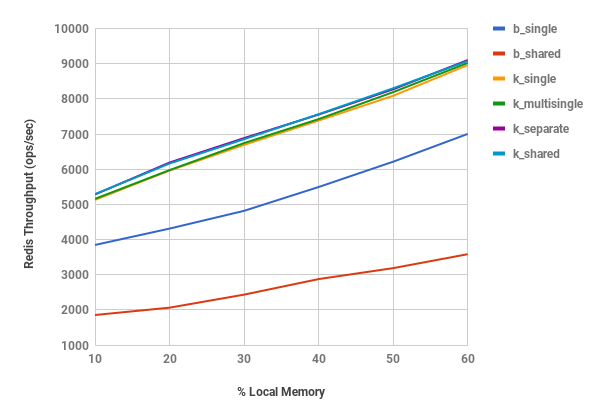
\includegraphics[width=\textwidth]{evaluation/compare_tp_redis.png}
		\caption{}
		\label{fig:compare_tp_redis}
	\end{subfigure}
	\caption{Redis performance comparison (Refer Table \ref{tab:graph_legends} for legends)}
	\label{fig:compare_redis}
\end{figure}

\begin{figure}[t]
	\centering
	
	\begin{subfigure}[t]{\textwidth}
		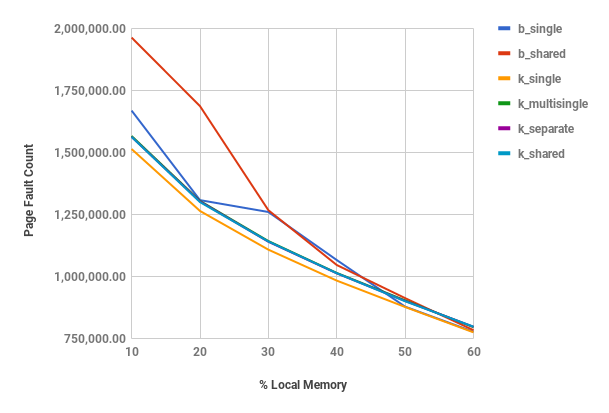
\includegraphics[width=\textwidth]{evaluation/compare_pf_memcached.png}
		\caption{}
		\label{fig:compare_pf_memcached}
	\end{subfigure}
	\begin{subfigure}[t]{\textwidth}
		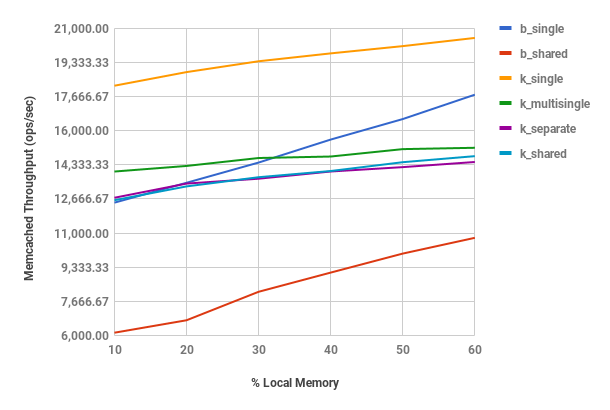
\includegraphics[width=\textwidth]{evaluation/compare_tp_memcached.png}
		\caption{}
		\label{fig:compare_tp_memcached}
	\end{subfigure}
	\caption{Memcached performance comparison (Refer Table \ref{tab:graph_legends} for legends)}
	\label{fig:compare_memcached}
\end{figure}


\chapter{Conclusion \& Future Work}

{\dime} provides good accuracy in terms of delay injection, local memory management and emulator isolation compared to existing emulators. We also show that it is capable of emulating real world applications and can be used to evaluate application performance in disaggregated memory environment. {\dime} allows fine grained partitioning of memory and flexibility to manage local memory with custom algorithms.

Since the disaggregated memory architecture is still in exploration phase, we will continue to add more features as the architecture evolves.

We plane to build a realistic emulator by involving more physical machines. A single machine will act as a remote memory blade and other servers will be able to map its memory into their own address space over RDMA.

%
\chapter{Materials and Methods}

\section{Including Figures}

Figures are conveniently included using postscript format.  If you are
generating a figure in a software, please check if the software
supports writing to a postscript or a PDF format. This format is loss
less vector format and with reproduce in any magnification without any
pixelation. Make sure to write it to an ``Encapsulated Post-script''or
.eps format.


\begin{figure}[tbp]
  \centering
    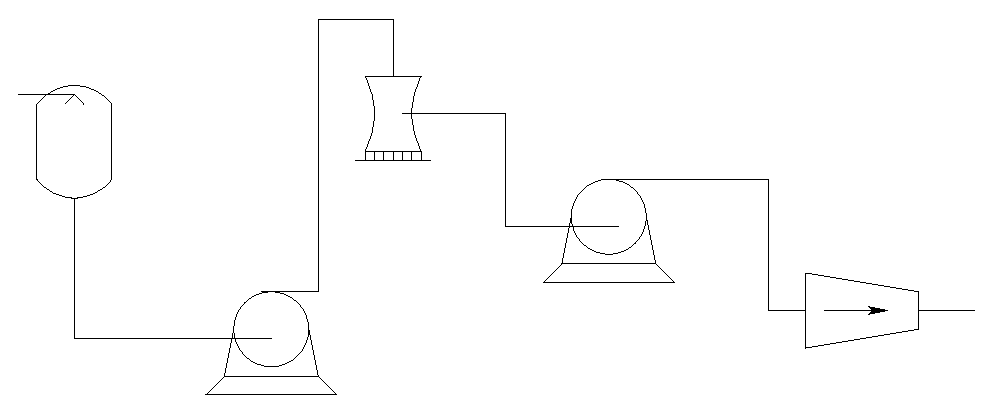
\includegraphics[width=0.7\textwidth]{profflow}
    \caption[Process flow sheet]{Process flow sheet of the
      experimental setup. The caption of the figure goes here. A
      shorter caption can be written in square brackets to identify it
      in the list of figures.}
    \label{fig:pfs} 
\end{figure}

Figures should be given a label and which can be used to refer to them
in the running text using \verb|\ref{}| command. Figure~\ref{fig:pfs}
describes the process flow sheet of the experimental set up used in
this report. The \Figref{fig:pfs} can also be refered by a short form notation
a pre-defined macro \verb"\Figref".



%%% Local Variables: 
%%% mode: latex
%%% TeX-master: "../mainrep"
%%% End: 

%\chapter{Results and Discussions}


\section{Including Tables}

Tables are to be used in a special environment so that they have a
Number, caption and appear in the list of tables.
Table~\ref{tab:samtab} is a sample table. In the case of tables, it is
a convention to write the caption above the table.  Note that in the
case of figures the caption appears below the figure.

\begin{table}[tbp]
  \centering
    \caption{Physical properties of the materials used.}
    \label{tab:samtab}
    \begin{tabular}{ll}
      \toprule 
      Property & Value \\
      \midrule
      Particle Density, $\rho_{\mathrm{p}}$ & 2500 kg/m$^{3}$ \\
      Viscosity, $\eta_{\mathrm{s}}$& 1 $\times 10^{-3}$ Pa-s \\
      \bottomrule \\
    \end{tabular}  
\end{table}

%%% Local Variables: 
%%% mode: latex
%%% TeX-master: "../mainrep"
%%% End: 


%******************************************************************
%                         Bibliography or References          
%******************************************************************  

\bibliographystyle{abbrv}
%\bibliographystyle{apalike}
%\bibliographystyle{sig-alternate}
\bibliography{mainrep}
    

%*******************************************************************
%                        Acknowledgements                    
%******************************************************************* 
%%%%
\acknowledgments

This section is for the acknowledgments. Please keep this brief and resist the temptation of writing flowery prose! Do include all those who helped you, e.g. other faculty/staff you consulted, colleagues who assisted etc.






\signature{\today}
%\signature[Indian Institute of Technology Bombay]{\today}

%========================================================================

%%% Local Variables: 
%%% mode: latex
%%% TeX-master: "../mainrep"
%%% End:            

%*******************************************************************
%                        About author                    
%*******************************************************************
%\colophon % remove this command while using this file.

% GAME OVER
%*******************************************************************
\end{document}

%%% Local Variables: 
%%% mode: latex
%%% TeX-master: t
%%% End: 
